\documentclass[11pt,a4paper,titlepage, ngerman]{article}

\usepackage[utf8]{inputenc}	% Diese Pakete sind
\usepackage[T1]{fontenc}		% für die Verwendung 
\usepackage{ngerman}			% von Umlauten im tex-file
\usepackage{lmodern}			% Schriftart, die am Bildschirm besser lesbar ist
\usepackage{graphicx}			% Zum Einbinden von Formeln
\usepackage{url}					% Zur Darstellung von Webadressen
\usepackage{siunitx}
\usepackage{amsmath}			% für equation*
\usepackage{subcaption}
\usepackage{wrapfig}

\begin{document}
%	\setlength{\parindent}{0em} 
	
	\begin{titlepage}
		\centering
		{\scshape\LARGE Versuchsbericht zu \par}
		\vspace{1cm}
		{\scshape\huge S2 -- Experimentieren, und dann?\par}
		\vspace{2.5cm}
		{\LARGE Gruppe 10 Mi\par}
		\vspace{0.5cm}
		{\large Alex Oster (E-Mail: a\_oste16@uni--muenster.de) \par}
		{\large Jonathan Sigrist (E-Mail: j\_sigr01@uni--muenster.de ) \par}
		\vfill
		durchgeführt am 25.10.2017\par
		betreut von\par
		{\large Dr. Anke \textsc{Schmidt}}
		
		\vfill
		
		{\large \today\par}
	\end{titlepage}
		
	\tableofcontents
	
	\newpage
	
	\section{Einleitung}
		\label{Einleitung}
		
		
		\glqq Die Gravitationskonstante $g$ besitzt in der Stadt Münster einen Wert von \SIrange{10,5}{11}{m/s^2}.\grqq
		
		Zu dieser Aussage führten die Ergebnisse einer Fallgeschwindigkeitsmessung an der WWU.
		Hierbei wurden die Geschwindigkeiten einer fallenden Metallkugel an zwei verschiedenen Punkten, mit Hilfe von Lichtschranken gemessen. Dadurch ließ sich die Fallbeschleunigung und damit die Gravitationskonstante bestimmen.
		
		Dieser neu gemessene Wert steht in Konflikt mit dem aktuellen Wert der PTB von $g = \SI{9.813}{\meter\per\second\squared}$ und es steht nun zur Diskussion, ob die PTB ihren derzeitigen Wert ändern muss.
		
		In diesem Bericht beschäftigen wir uns damit, diese Aussage zu widerlegen.
		Dazu messen wir die Zeit von Pendelschwingungen und berechnen aus Fadenlänge und gemessener Zeit die Gravitationskonstante. Um ein möglichst genaues Ergebnis zu erhalten, führen wir mehrere Messungen mit verschiedenen Fadenlängen durch.
		
	\section{Methoden}
		Die Gravitationskonstante $g$ wurde durch das Modell des mathematisch idealisierten Pendels berechnet\footnote{Weitere Erläuterungen in (\ref{pendel} Mathematisches Pendel).}.
		Für unsere Messung haben wir eine an einem Faden befestigte Metallkugel verwendet. Der Faden war dabei an einer starren Halterung angebracht und seine Länge $L$ ließ sich beliebig einstellen.
		
		\begin{figure}[ht]
			\centering
			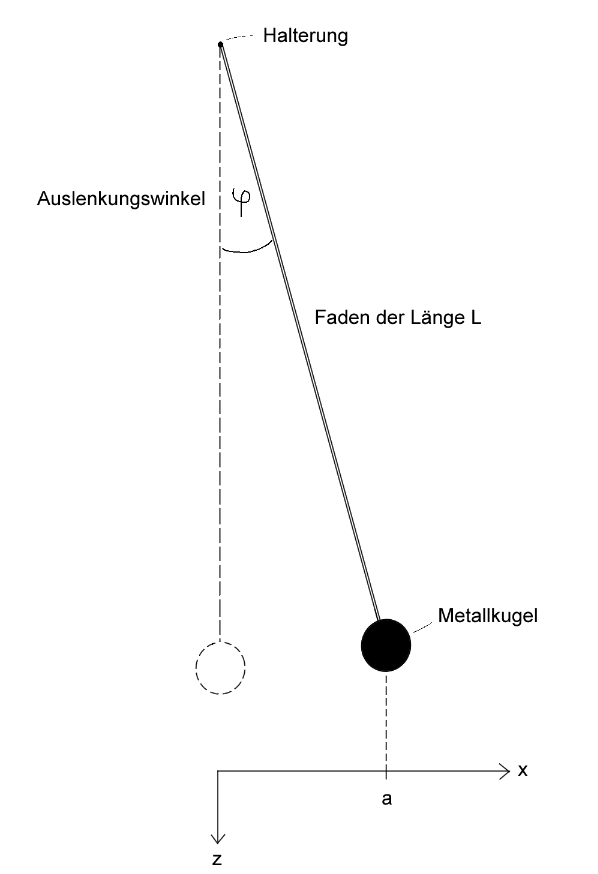
\includegraphics[scale=0.4]{Pendel.png}		
			\caption{Versuchsskizze}
			\label{fig:pendel}
		\end{figure}
		
		Wie in Abb. \ref{fig:pendel} dargestellt, wurde die Kugel am Punkt $x = a$ unter einer kleinen Auslenkung $\varphi_0$ losgelassen.
		Wsir haben die Zeit gemessen, welche die Metallkugel benötigt hat, um eine bestimmte Anzahl Schwingung zu durchlaufen, also bis die Metallkugel wieder bei ca. $x = a$ angekommen ist.
		Das war gerade dann der Fall wenn die Kugel ihre Bewegungsrichtung gewechselt hat und somit leicht abzuschätzen.
		Wir haben jeweils mehrere Schwingungen in einer Messung zusammengefasst, um die Ungenauigkeiten von der Zeitmessung möglichst klein zu halten. 
		
		Die Zeit wurde mit einer handelsüblichen digitalen Stoppuhr gemessen, welche zwei Nachkommastellen anzeigt.
		Eine Ungenauigkeit der Uhr ist uns nicht bekannt.
		Zum Messen der Seillänge haben wir ein Maßband von zwei Metern Länge benutzt. Die Millimeter-angaben konnten leicht abgelesen werden.
		Auch hier ist uns eine Ungenauigkeit des Maßstabes nicht bekannt.
		Die Kugel hatte einen Durchmesser von \SI{3}{\cm}.
		
		Für zwei Fadenlängen wurden viele Schwingungen gemessen und für vier weitere weniger.
		Dadurch konnten zusätzliche Referenzwerte geliefert werden, welche ebenfalls gegen die Behauptung gehen.
		
	\section{Durchführung}
		\label{Durchführung}
		
		
		\subsection{Messung}
		\label{Messung}
			Es folgen durchschnittliche Zeiten für die Periodendauern, welche sich durch die durchgeführten Messungen für verschiedene Fadenlängen $L$ ergaben: 
			\vspace{0.25cm} 
			
			\begin{description}
				
				\item[Fadenlänge 1:]($L = \SI{111,6}{cm}$)\\
				Für die erste Fadenlänge haben wir 110 Schwingungsdauern in 10er Schritten gemessen. (D.h. jeweils die Periodendauer für zehn Schwingungen auf einmal) \\
				Die durchschnittliche Zeit für eine Pendelschwingung betrug hierbei: \SI{2.134}{s}
				
				\item[Fadenlänge 2:]($L = \SI{104,5}{cm}$)\\ 				 
				Bei dieser und der folgenden Messung haben wir nur 20 Perioden, in 5er Schritten, gemessen. Hier betrug die durchschnittliche Zeit für eine Pendelschwingung: \SI{2,060}{s}
				
				\item[Fadenlänge 3:]($L = \SI{86,9}{cm}$)\\ 			
				Wie auch bei der vorherigen Messung wurden hier nur 20 Schwingungen betrachtet. Dabei ergab sich, für eine Pendelschwingung, die durchschnittliche Zeit: \SI{1,879}{s}		
				
				\item[Fadenlänge 4:]($L = \SI{65,8}{cm}$)\\ 				
				Diese Messung und die Folgende betrachten wir 25 Perioden, ebenfalls in 5er Schritten. Die durchschnittliche Zeit für eine Pendelschwingung betrug hierbei: \SI{1,876369}{s}
				
				\item[Fadenlänge 5:]($L = \SI{116,3}{cm}$)\\ 				
				Hier erhalten wir für eine Pendelschwingung die durchschnittliche Zeit: \SI{2,174}{s}
				
				\item[Fadenlänge 6:]($L = \SI{92,6}{cm}$)\\ 				
				Da wir bei den letzten vier Messungen nicht viele Schwingungen betrachtet haben, haben wir für die sechste Fadenlänge noch einmal 100 Schwingungsdauern gemessen. Dabei haben wir eine Länge $L$ gewählt, die circa \SI{20}{cm} von der ersten abwich, um mehrere Werte für \glqq deutlich\grqq unterschiedliche Längen $L$ zu erhalten. 
				Hierbei betrug die durchschnittliche Zeit für eine Pendelschwingung: \SI{1,936}{s}
				
			\end{description}
		
	\section{Diskussion}	
		\label{Diskussion}		
		
		\subsection{Mathematisches Pendel}
		\label{pendel}
		
			%%%%Die Bewegungsbahn der Kugel kann recht gut abgeschätzt werden %kleinere ungenauigkeiten Wir schätzen nicht, wir rechnen bzw. nähern
			Wir betrachten für die Auswertung unserer Messungen das Modell des mathematischen Pendels unter folgenden Annahmen:
			
			\begin{enumerate}
				\item Die gesamte Masse $m$ ist im Schwerpunkt vereinigt (Massepunkt).
				\item Der Massepunkt m ist durch einen masselosen Faden oder alternativ durch eine masselose starre Verbindung der Länge $L$ mit dem Aufhängepunkt verbunden.
				\item Die Bewegung erfolgt ohne Reibung.
				\item Das Pendel wird nur leicht ausgelenkt %langsam und $\alpha$ ist klein.
			\end{enumerate}
			
			\begin{figure}[ht]
				\centering
				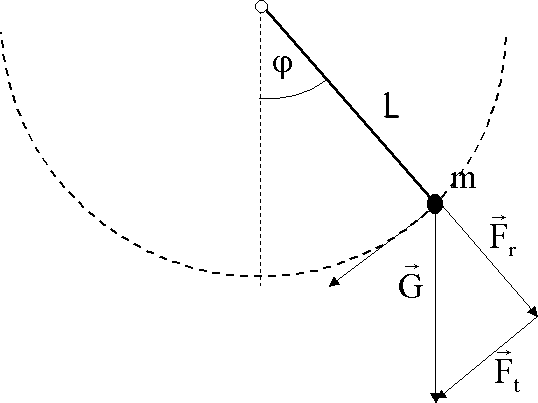
\includegraphics[scale=0.4]{mathematischesPendel.png}		
				\caption{mathematisches Pendel}
				\label{fig:matpendel}
			\end{figure}
			
			\setlength{\parindent}{0em}
				Auf den Massepunkt m wirkt die Schwerkraft $ \vec{G}$ bzw. $ \vec{F_\textsc{g}}$ (vgl. Abbildung \ref{fig:matpendel}) \\
			
			\begin{center}
				{ $ \vec{F_\textsc{g}} = m\vec{g}$} 
			\end{center}
			
			Nur die Tangentialkompenente $F_\varphi$ der angreifenden Kraft $ \vec{F_\textsc{g}}$ ist für die Bewegung des Massepunktes entlang des Kreisbogens verantwortlich.   	
			  
			$F_\varphi$ ist der Auslenkung $\varphi$ entgegen gerichtet und wirkt  rücktreibend auf den Massepunkt:
			
			\begin{center}  
				$F_\varphi = - m\vec{g} \sin\varphi.$ 
			\end{center}
			
			Mit den Gleichungen 
			\begin{center}
				$a = L \ddot{\varphi}$ und $F = ma$ 
			\end{center}
		
			ergibt sich die Bewegungsgleichung eines frei schwingenden Fadenpendels: 
			\begin{center}
				$\ddot{\varphi}+\left( \frac{g}{L}\right)  \sin \varphi = 0$	
			\end{center}
			
			Diese nichtlineare Differentialgleichung zweiter Ordnung vereinfachen wir mit der Kleinwinkelnäherung
			\begin{center}
				$\sin \varphi \approx \varphi $	
			\end{center} 
			
			Somit haben wir nun eine dem harmonischen Oszillator entsprechende DGL:
			\begin{center}
				$\ddot{\varphi}+\frac{g}{L} \varphi = 0$	
			\end{center}
			
			Die Frequenz lässt sich hierbei einfach bestimmen: 
			\begin{center}
				$\omega =  \sqrt{\frac{g}{L}}$
			\end{center}
			
			Damit ist die Periodendauer:
			\begin{center}
				$T =  2\pi \sqrt{\frac{L}{g}}$
			\end{center} 
		
			Die Schwingungsdauer ist also unabhängig von der Masse und unsere Gravitationskonstante $g$ bestimmt sich wie folgt:
			\begin{center}
				$g = (\frac{2 \pi}{T})^2 L$
			\end{center} 
		
		\subsection{Datenanalyse}
		\label{Auswertung}	
	
			Die Ergebnisse der beiden genaueren Messungen sind in Abb. \ref{fig:seilKonst} dargestellt.
			Hierbei beschreiben \glqq Messung 1/2\grqq {} die erste/zweite genauere Messung (Fadenlänge 1 bzw. 6).
			Auffällig ist, dass die Streuung bei Messung 2 deutlich geringer war.
			
			Unsere Messwerte angewandt auf die obige Gleichung für $g$ ergaben unter Berücksichtigung der Messungenauigkeiten folgende Werte:
			
			\begin{table}
				\label{Tab:WerteTabelle}
				\centering
				\begin{tabular}{l|S|S|S}
					\hline
					& {Messung 1} & {Messung 2} & {restliche Messungen (Mehrfachmessung)} \\ \hline
					$g$ &  &  & \\ \hline %TODO
				\end{tabular}
				\caption{Ergebnisse der Messungen}
			\end{table}
			
			Diese Werte deuten eindeutig darauf hin, dass die Gravitationskonstante nicht im Bereich von \SIrange{10,5}{11}{m/s^2} liegt, da alle Messwerte nahe dem Literaturwert liegen und die Streuung nicht bis \SI{10,5}{m/s^2} kommt.
			So stellt sich die Frage, welche Faktoren Einfluss auf die Lichtschrankenmessung hatten, so dass sich Werte von $g$ in diesem Bereich ergaben. 
							
			\begin{figure}[ht]
				\begin{subfigure}{0.5\textwidth}
					\centering
					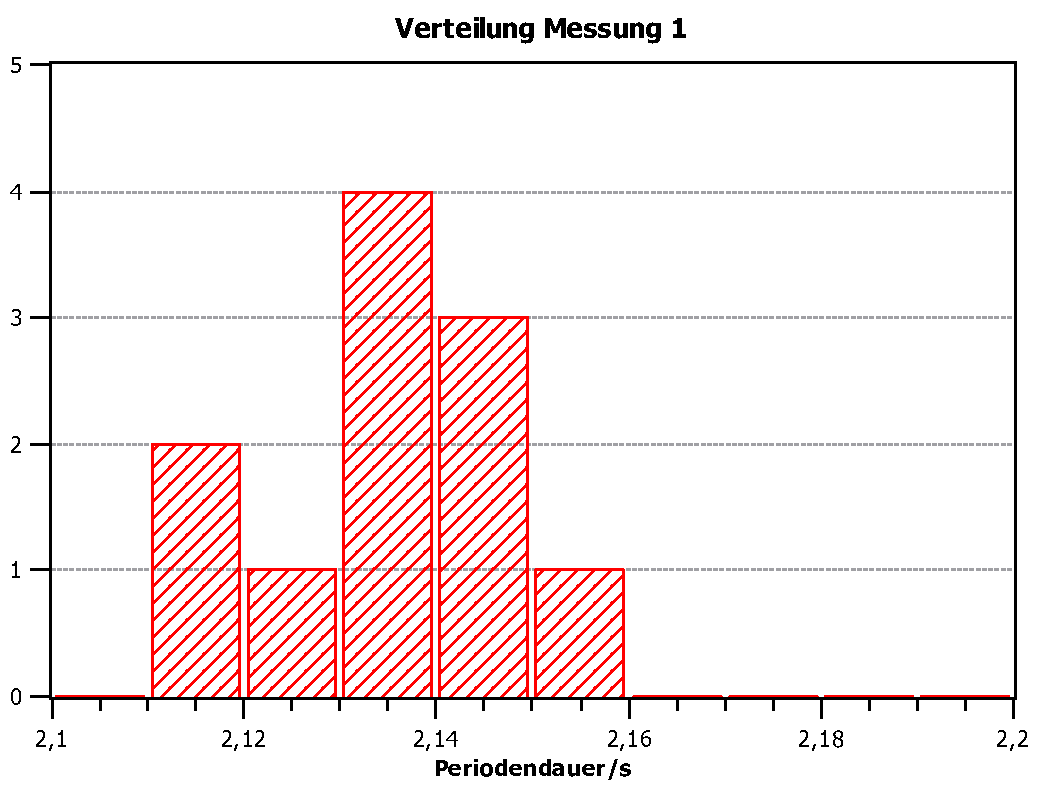
\includegraphics[scale=0.35]{VerteilungMessung1.pdf}
				\end{subfigure}
				\begin{subfigure}{0.5\textwidth}
					\centering
					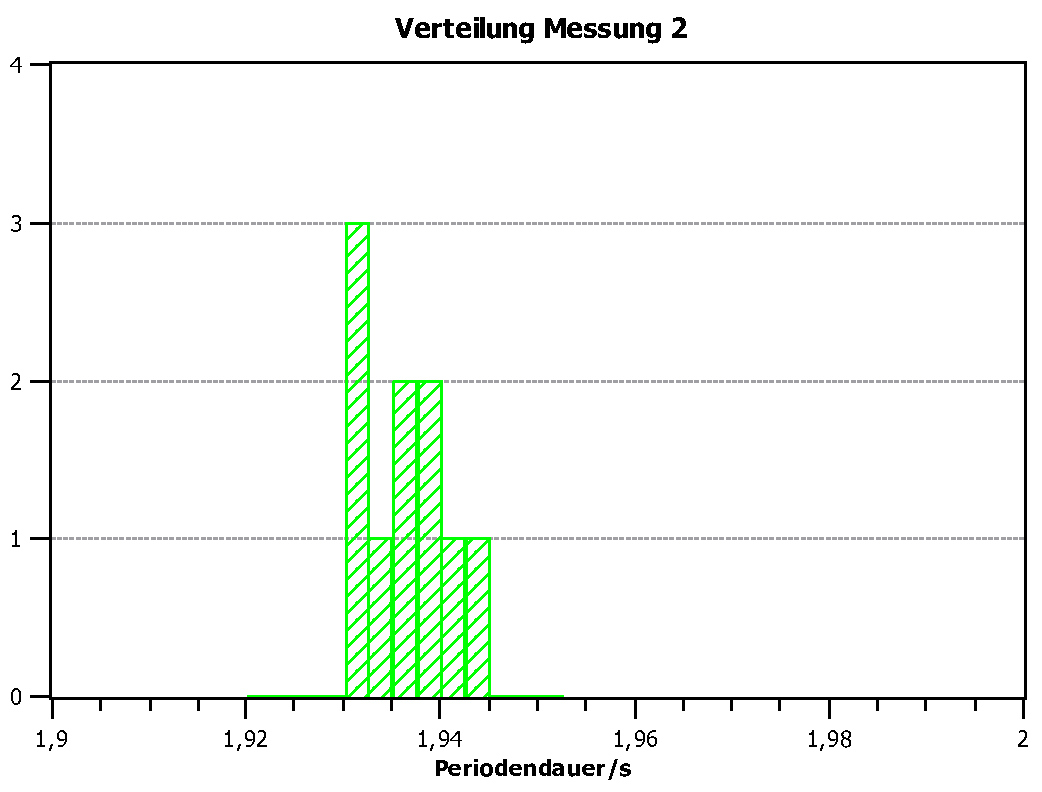
\includegraphics[scale=0.35]{VerteilungMessung2.pdf}
				\end{subfigure}		
				\caption{Messergebnisse bei konstanter Seillänge}
				\label{fig:seilKonst}
			\end{figure}
		
		\begin{thebibliography}{9}		
			\item[Abbildung 2:] \url{http://people.physik.hu-berlin.de/~mitdank/dist/scriptenm/pendel-Dateien/image001.gif}			
		\end{thebibliography}	
			
\end{document} 